\documentclass[12pt]{exam}

\usepackage[margin=0.75in]{geometry}
\usepackage{amsmath,amssymb,amsthm, graphicx}
\usepackage{braket} % provides \ket{}, \bra{}, \braket{}, etc.
\printanswers
\setlength{\parindent}{0pt}

\begin{document}

\title{CSE 4412: Quantum Computing Prog 1}
\author{Gordon Chen, gbc24001}
\date{}
\maketitle

\section{Problem 1}
\textbf{One-qubit operations.} Construct a circuit that starts with $\lvert 0\rangle$
and then apply an H gate followed by a Z gate.

\begin{enumerate}
    \item Calculate yourself the output state of the circuit.
        \begin{solution}\\
            $Z H \ket{0} = Z \ket{+} = \frac{1}{\sqrt{2}} Z (\ket{0} + \ket{1})
            = \frac{1}{\sqrt{2}} (\ket{0} - \ket{1}) = \boxed{\ket{-}}$
        \end{solution}

    \item Describe the visualization results from the Composer, in particular, the probability
        amplitude and state vector. Verify that what you see in the composer is consistent
        with your own calculation.

        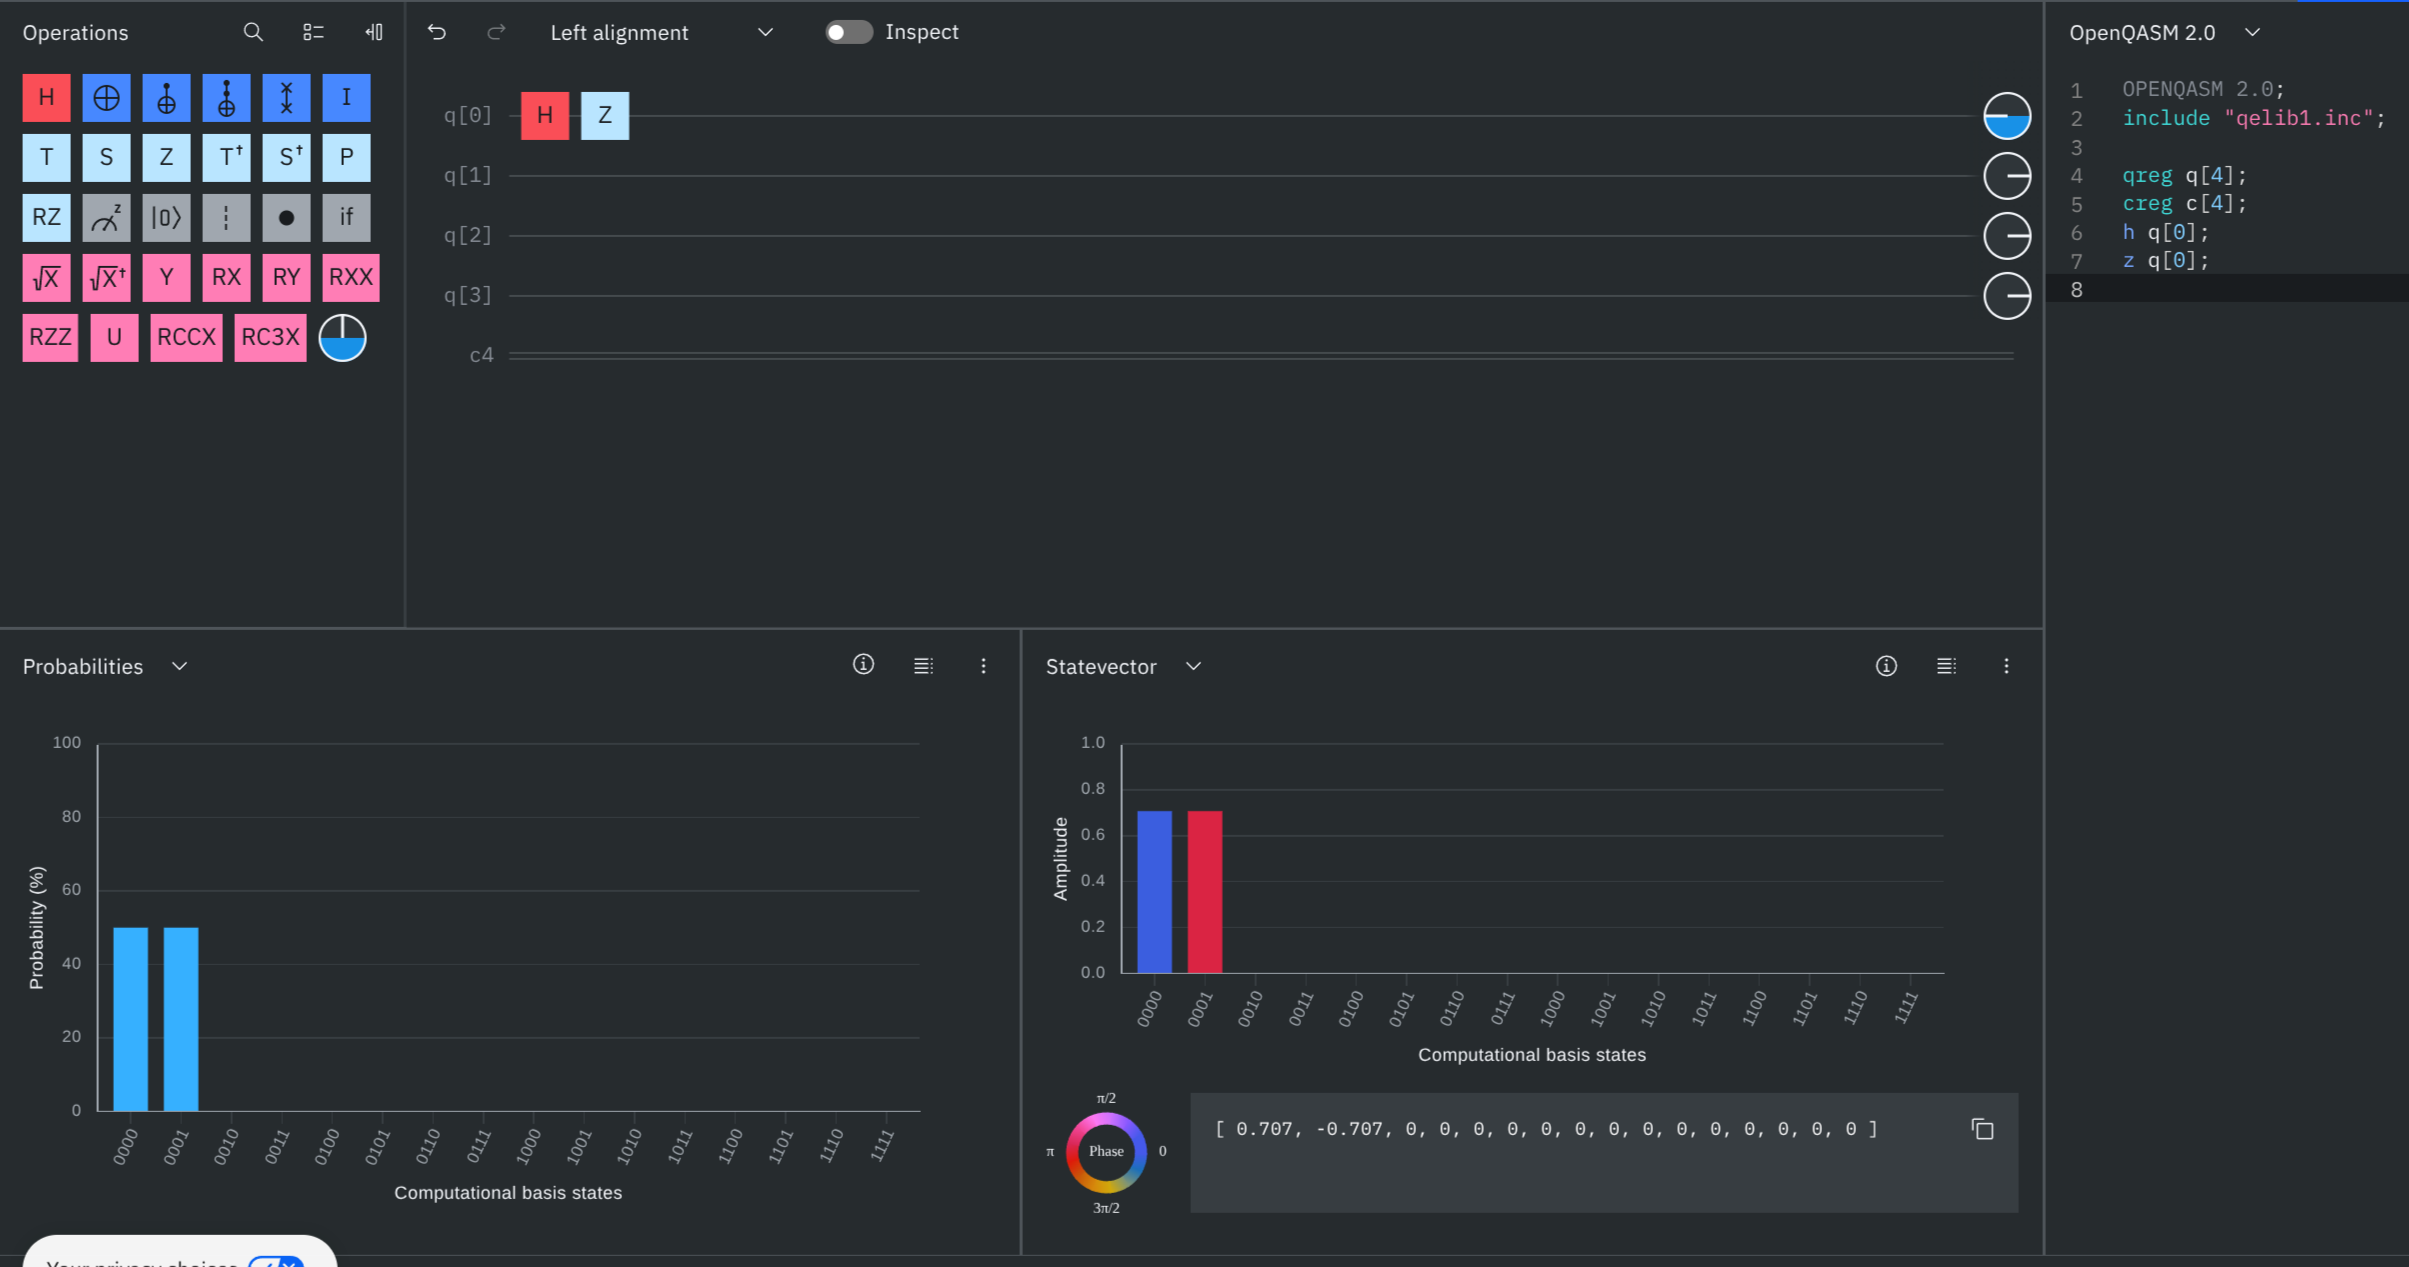
\includegraphics[width=\linewidth]{imgs/p1.png}

        \begin{solution}\\
            The probability amplitudes are $\frac{1}{2}$ for $\ket{0000}$ and $\ket{0001}$.
            State vector is $\frac{1}{\sqrt{2}}(\ket{0000} - \ket{0001})$.
            This matches what I calculated because $\ket{-} = \frac{1}{\sqrt{2}}(\ket{0} - \ket{1})$
            so $\mathbb{P}(\ket{0}) = \mathbb{P}(\ket{1}) = \frac{1}{2}$.
        \end{solution}

\end{enumerate}

\section{Problem 2}
\textbf{Entanglement.} In class, we have constructed a circuit in IBM Quantum Composer
that outputs Bell state $\lvert \Phi^{+}\rangle$ (Bell state is also called EPR pair). In this problem, you
will use the Composer to construct circuits that output the other three Bell states
$\lvert \Phi^{-}\rangle$, $\lvert \Psi^{+}\rangle$, and $\lvert \Psi^{-}\rangle$.
The Bell states are prime examples of entangled states (see HW1 for the definitions of these states!).

$$\ket{\Phi^{+}}=\frac{1}{\sqrt{2}}\bigl(\ket{0,0}+\ket{1,1}\bigr),\qquad
\ket{\Phi^{-}}=\frac{1}{\sqrt{2}}\bigl(\ket{0,0}-\ket{1,1}\bigr),$$

$$\ket{\Psi^{+}}=\frac{1}{\sqrt{2}}\bigl(\ket{0,1}+\ket{1,0}\bigr),\qquad
\ket{\Psi^{-}}=\frac{1}{\sqrt{2}}\bigl(\ket{0,1}-\ket{1,0}\bigr).$$

\begin{enumerate}
    \item You will construct three circuits, for $\lvert \Phi^{-}\rangle$,
        $\lvert \Psi^{+}\rangle$, and $\lvert \Psi^{-}\rangle$, respectively. For each
        circuit, briefly describe your thoughts in designing the circuit.

        \begin{solution}\\
            $\ket{\Phi^+} = \mathrm{CNOT} \ H \ket{00} = \mathrm{CNOT} \ket{+0}$
            $= \frac{1}{\sqrt{2}} \mathrm{CNOT} (\ket{0} + \ket{1}) \otimes \ket{0}$

            $= \frac{1}{\sqrt{2}} \mathrm{CNOT} (\ket{00} + \ket{10})$
            $= \frac{1}{\sqrt{2}} (\ket{00} + \ket{11})$\\


            For $\ket{\Phi^-}$ we basically want the same thing as $\ket{\Phi^+}$,
            except we need flip phase of the $\ket{11}$. We can do this by using a $Z$ gate.

            $\ket{\Phi^-} = (Z \otimes I) \ket{\Phi^+}$
            $=(Z \otimes I) (\frac{1}{\sqrt{2}} (\ket{00} + \ket{11})$
            $=\frac{1}{\sqrt{2}} (\ket{00} - \ket{11})$

            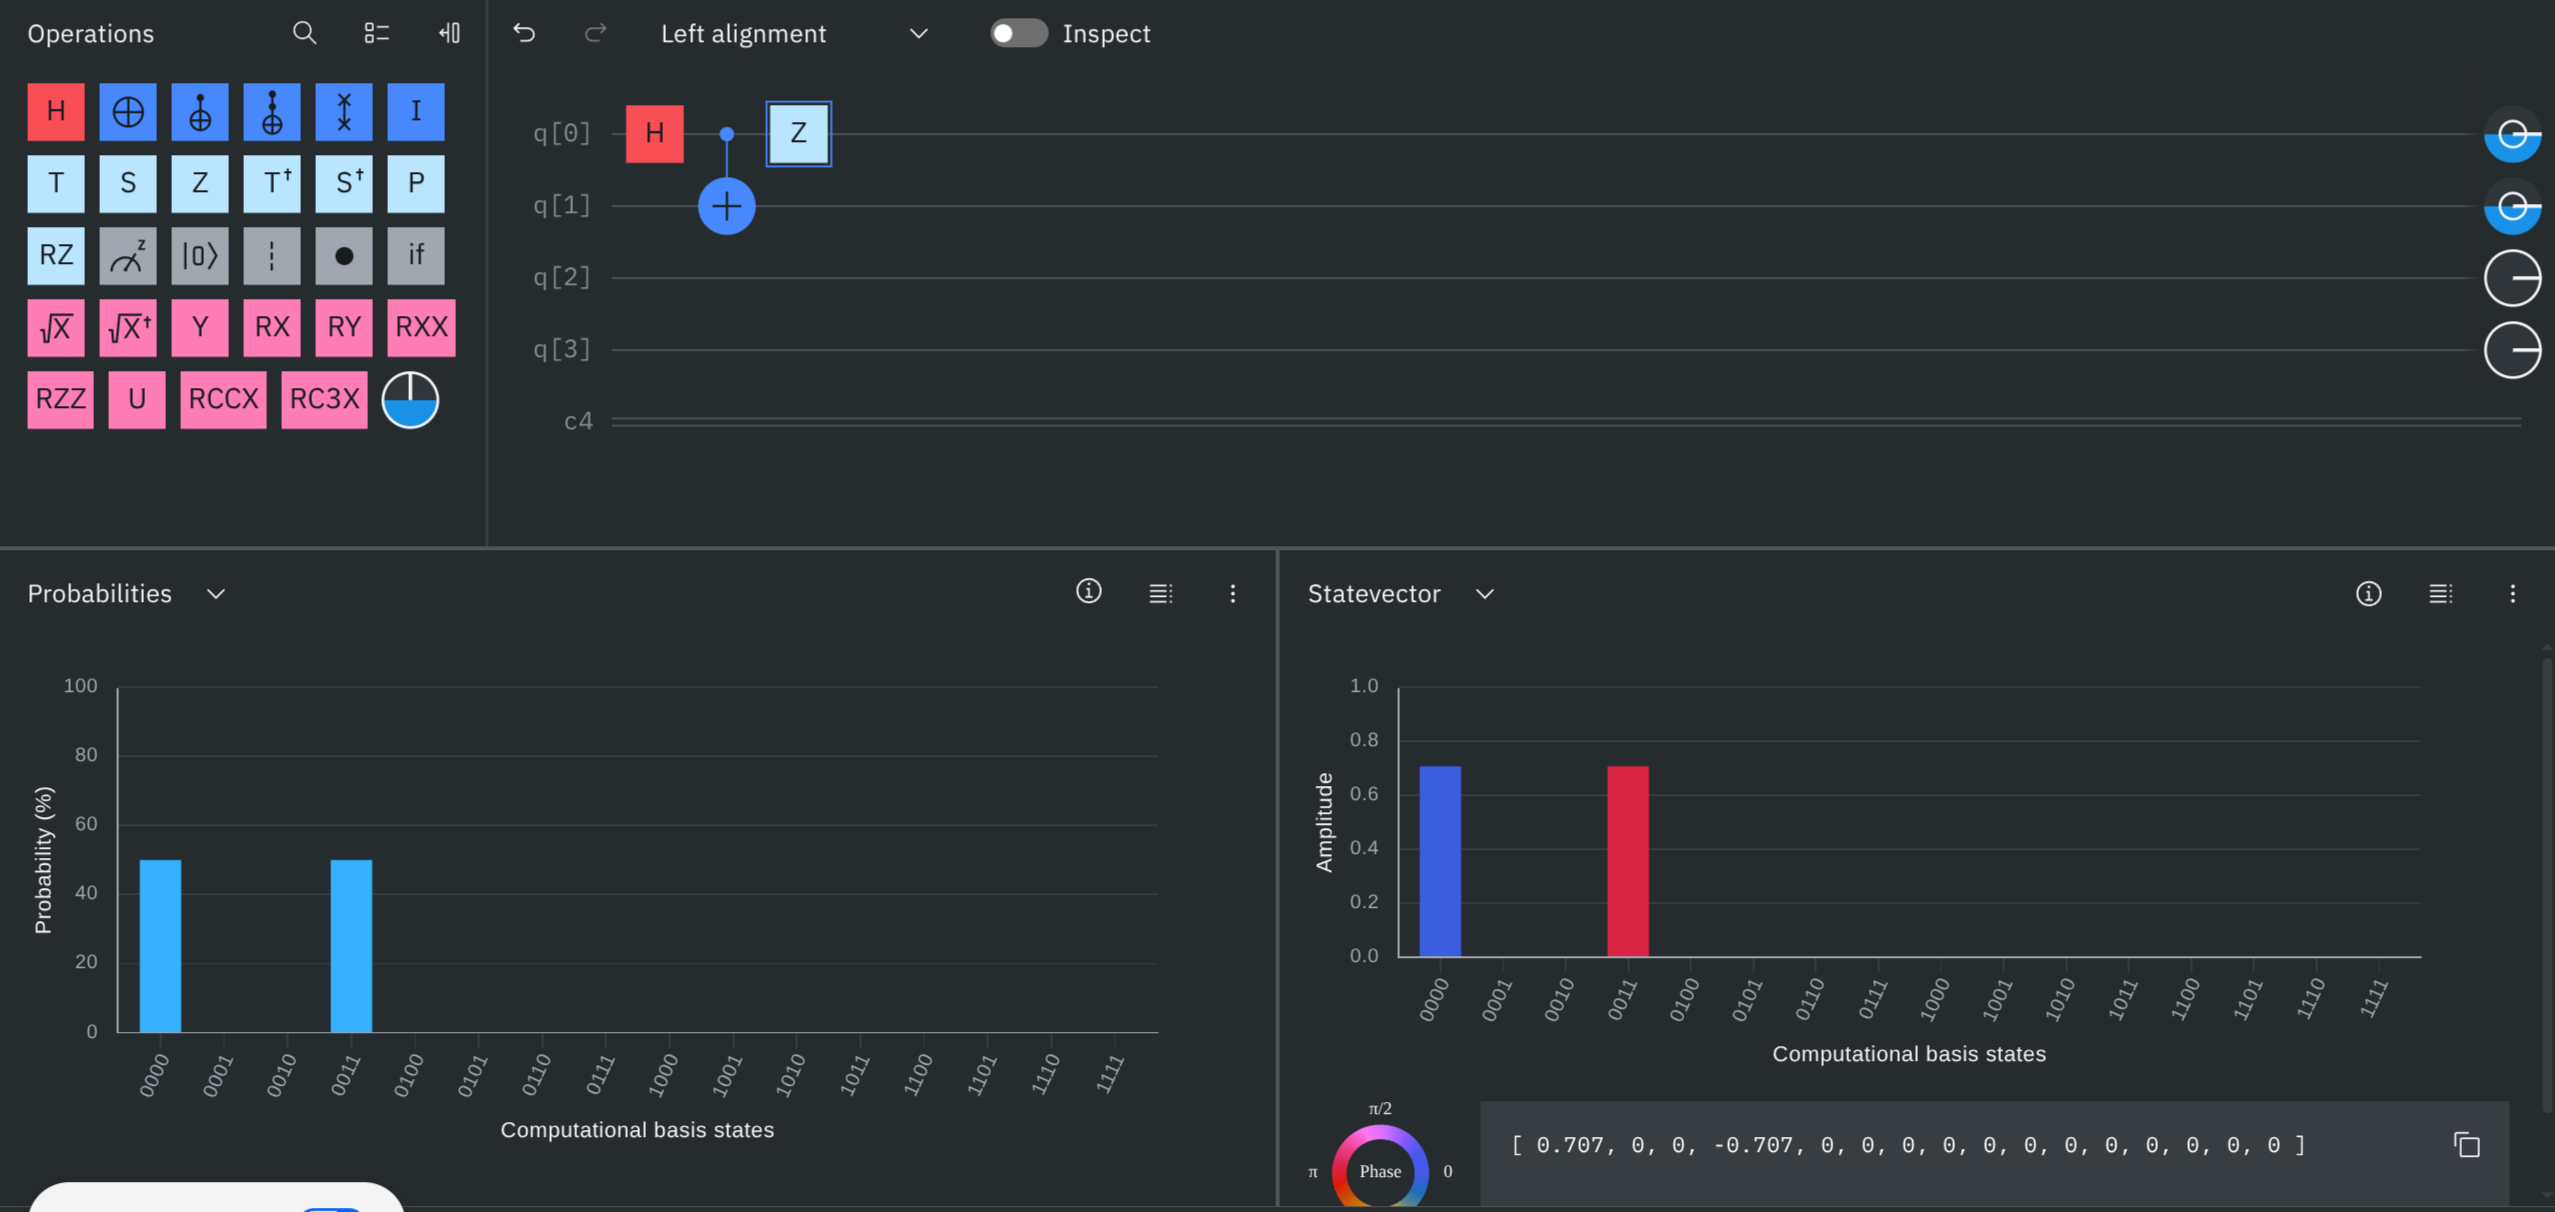
\includegraphics[width=\linewidth]{imgs/p2_phi_minus.png}\\\\


            For $\ket{\Psi^+}$ we just need to flip the second register of $\ket{\Psi^+}$.
            We can use an $X$ gate for that.

            $\ket{\Psi^+} = (I \otimes X) \ket{\Phi^+}$
            $= (I \otimes X) (\frac{1}{\sqrt{2}} (\ket{00} + \ket{11})$
            $=\frac{1}{\sqrt{2}} (\ket{01} + \ket{10})$

            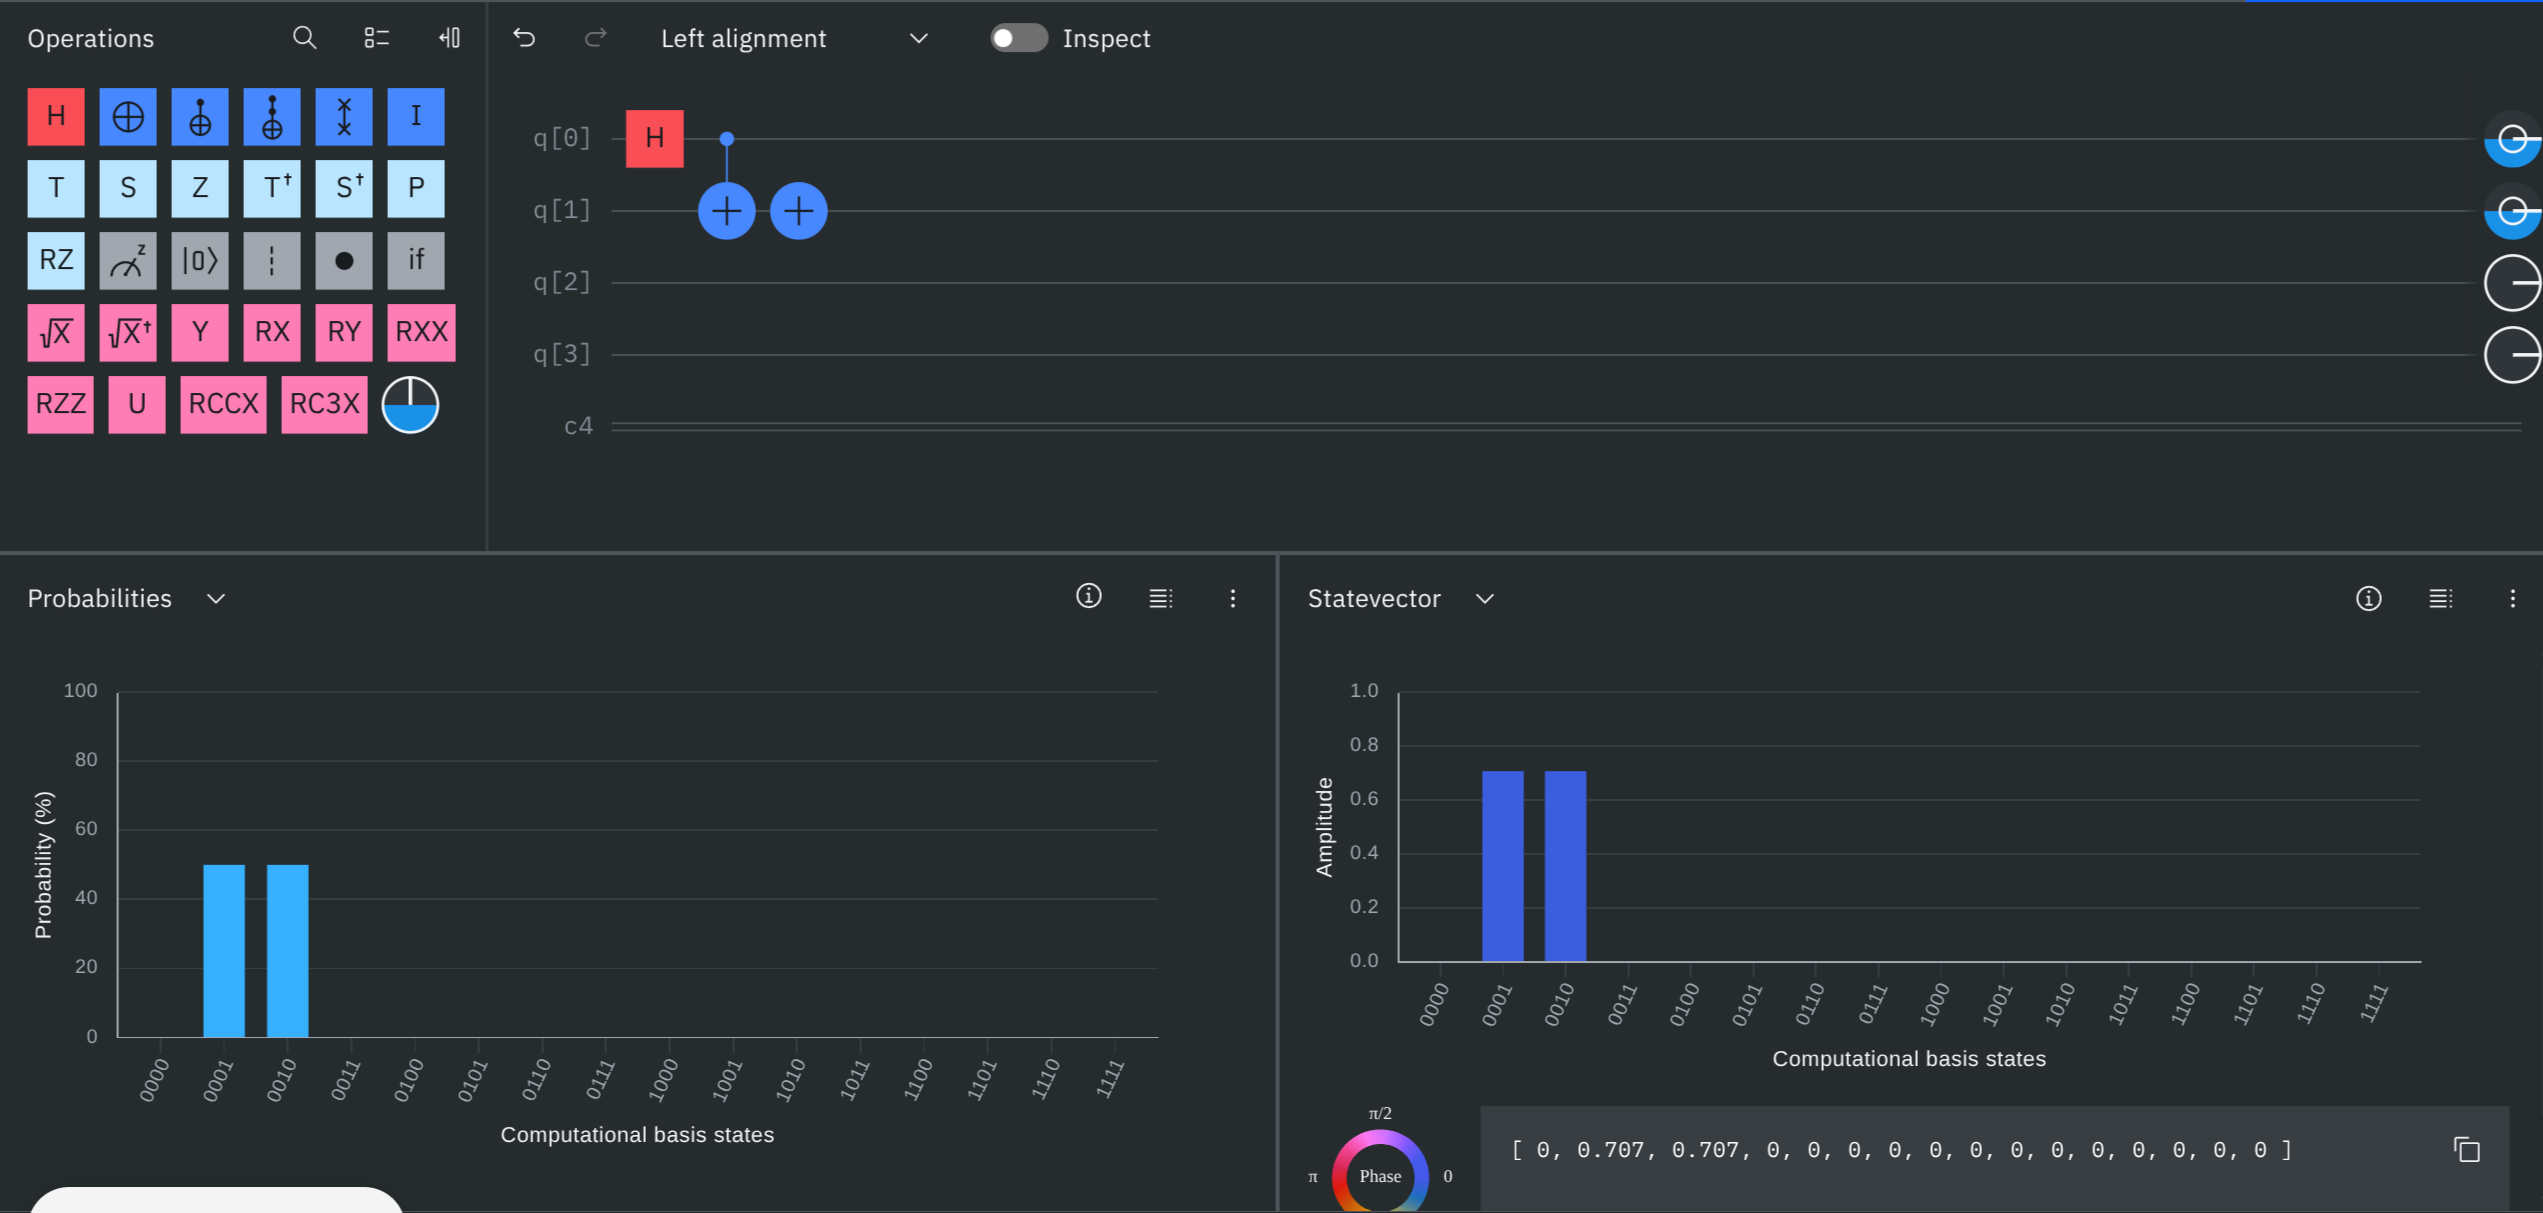
\includegraphics[width=\linewidth]{imgs/p2_psi_plus.png}\\\\


            For $\ket{\Psi^-}$ we just need to flip the sign of $\ket{\Psi^+}$.
            We can use an $Z$ gate for that.

            $\ket{\Psi^-} = (Z \otimes I) \ket{\Psi^+}$
            $= (Z \otimes I) (\frac{1}{\sqrt{2}} (\ket{01} + \ket{10})$
            $=\frac{1}{\sqrt{2}} (\ket{01} - \ket{10})$

            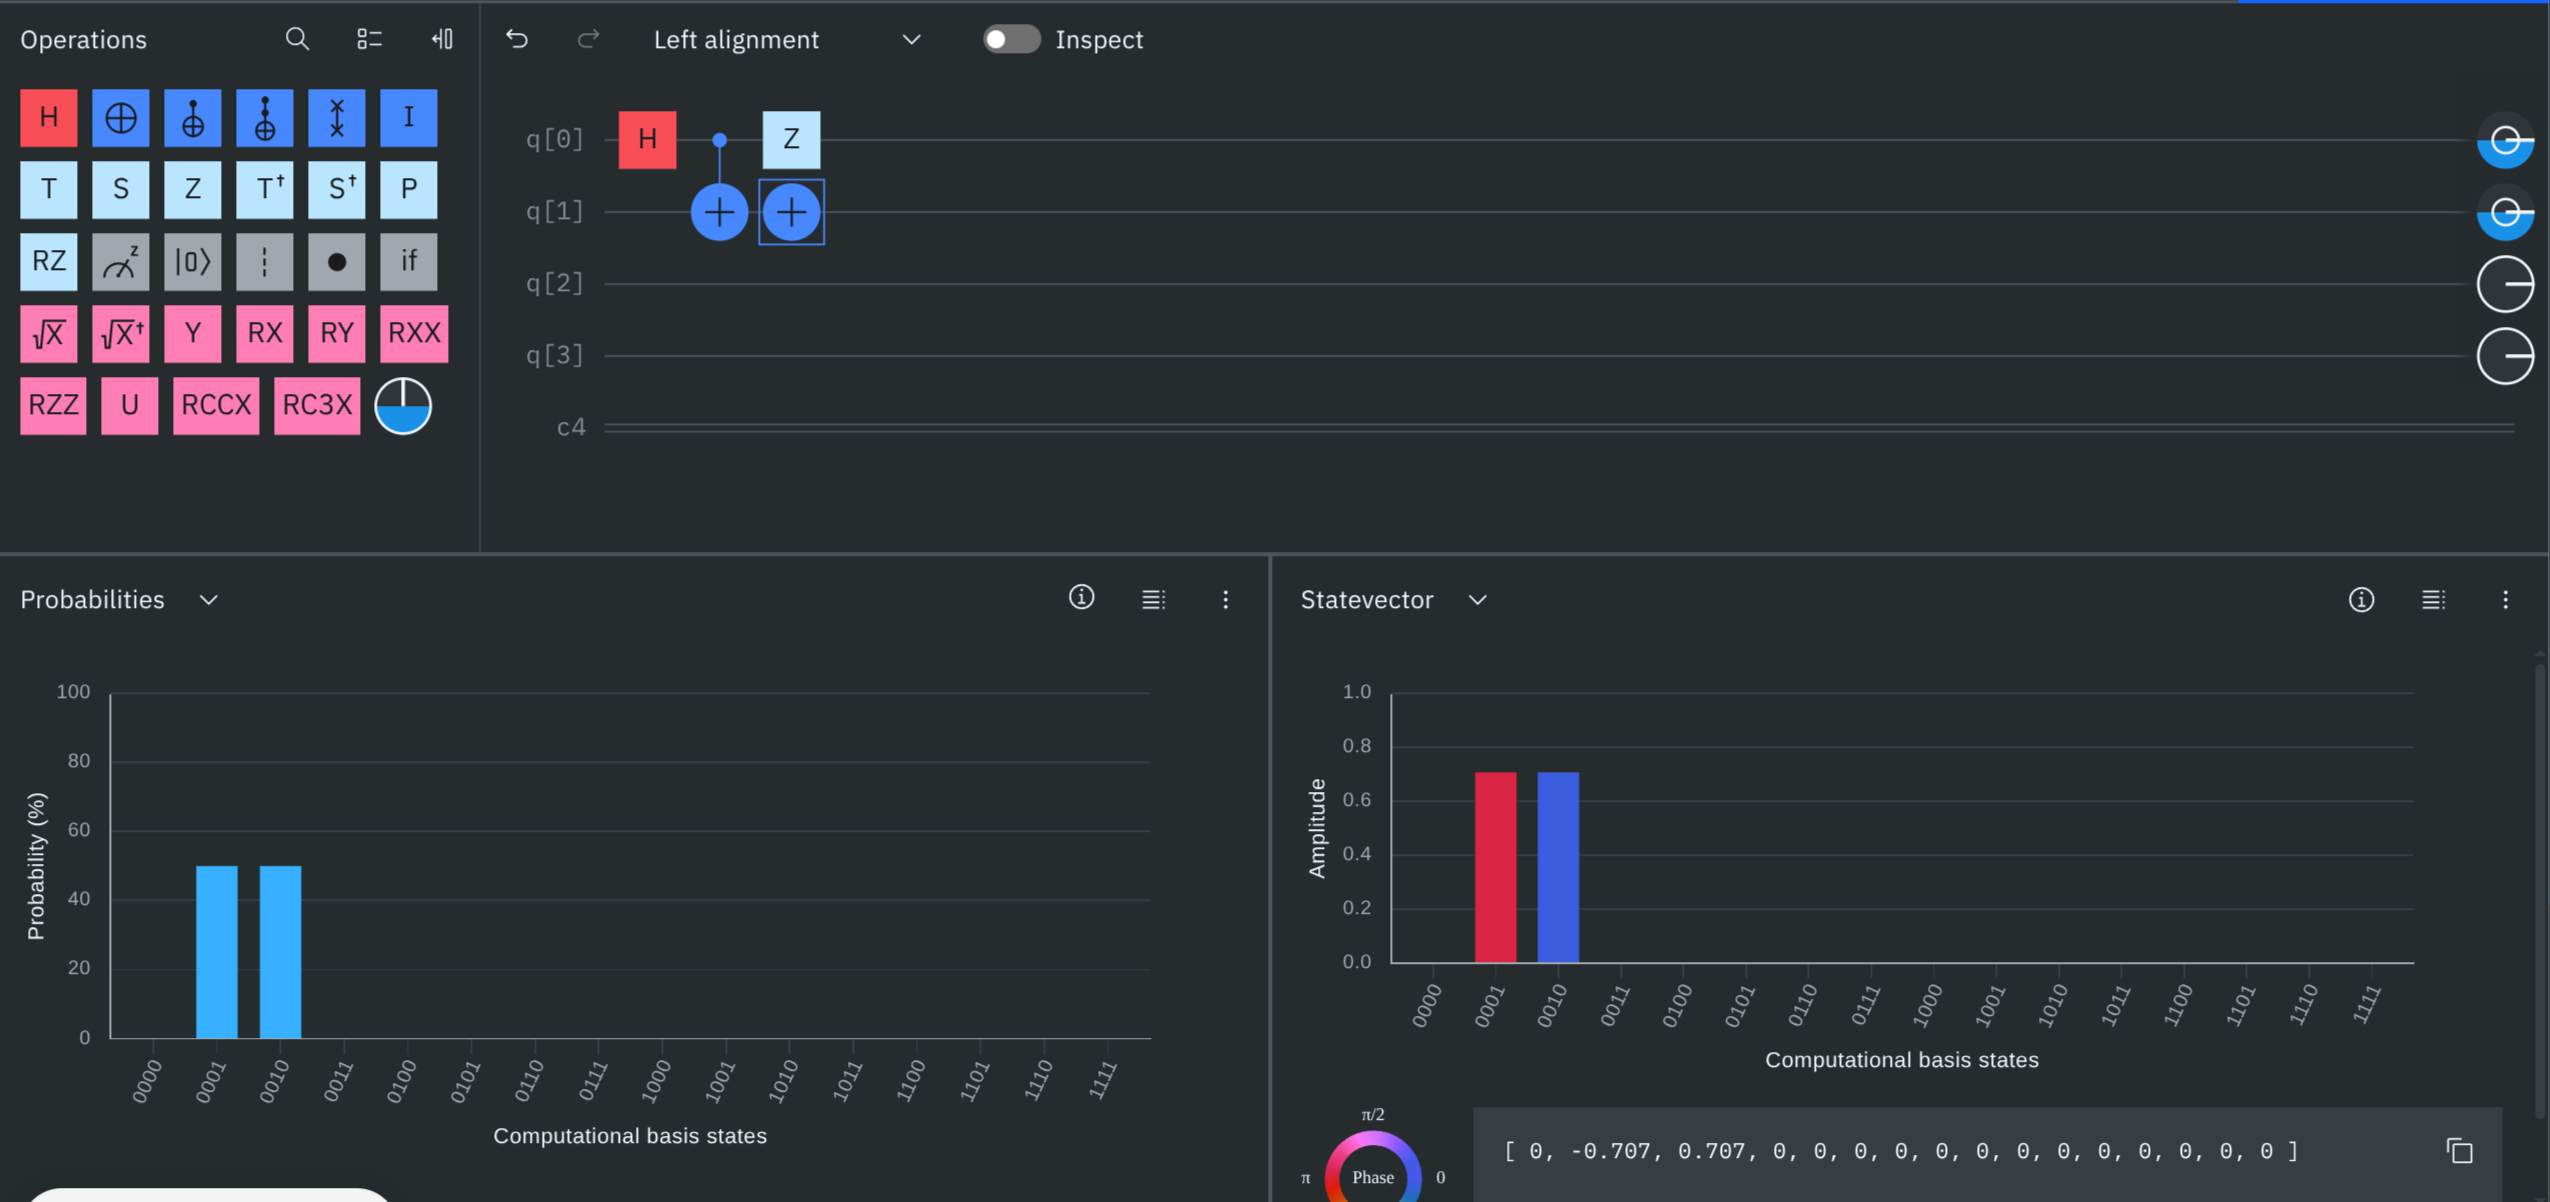
\includegraphics[width=\linewidth]{imgs/p2_psi_minus.png}
        \end{solution}

    \item Use the visualization in the Composer to convince yourself that your design indeed
        provides the desired output.
\end{enumerate}

\section{Problem 3}
\textbf{CNOT gate.} What is the resulting quantum state after applying the following operations:

$$\mathrm{CNOT}(H \otimes H)\lvert +, 0\rangle$$

Write your answer in the Z basis! Construct a circuit in IBM Composer for the above
operations. Use the output from the Composer to verify your answer.

\begin{solution}\\\\
$\mathrm{CNOT} (H \otimes H) \ket{+, 0}$\\

$ = \mathrm{CNOT} \ket{0, +}$\\

$ = \mathrm{CNOT} (\ket{0} \otimes \frac{1}{\sqrt{2}}(\ket{0} + \ket{1}))$\\

$ = \frac{1}{\sqrt{2}} \mathrm{CNOT} (\ket{00} + \ket{01})$\\

$ = \boxed{\frac{1}{\sqrt{2}} (\ket{00} + \ket{01})}$
\end{solution}

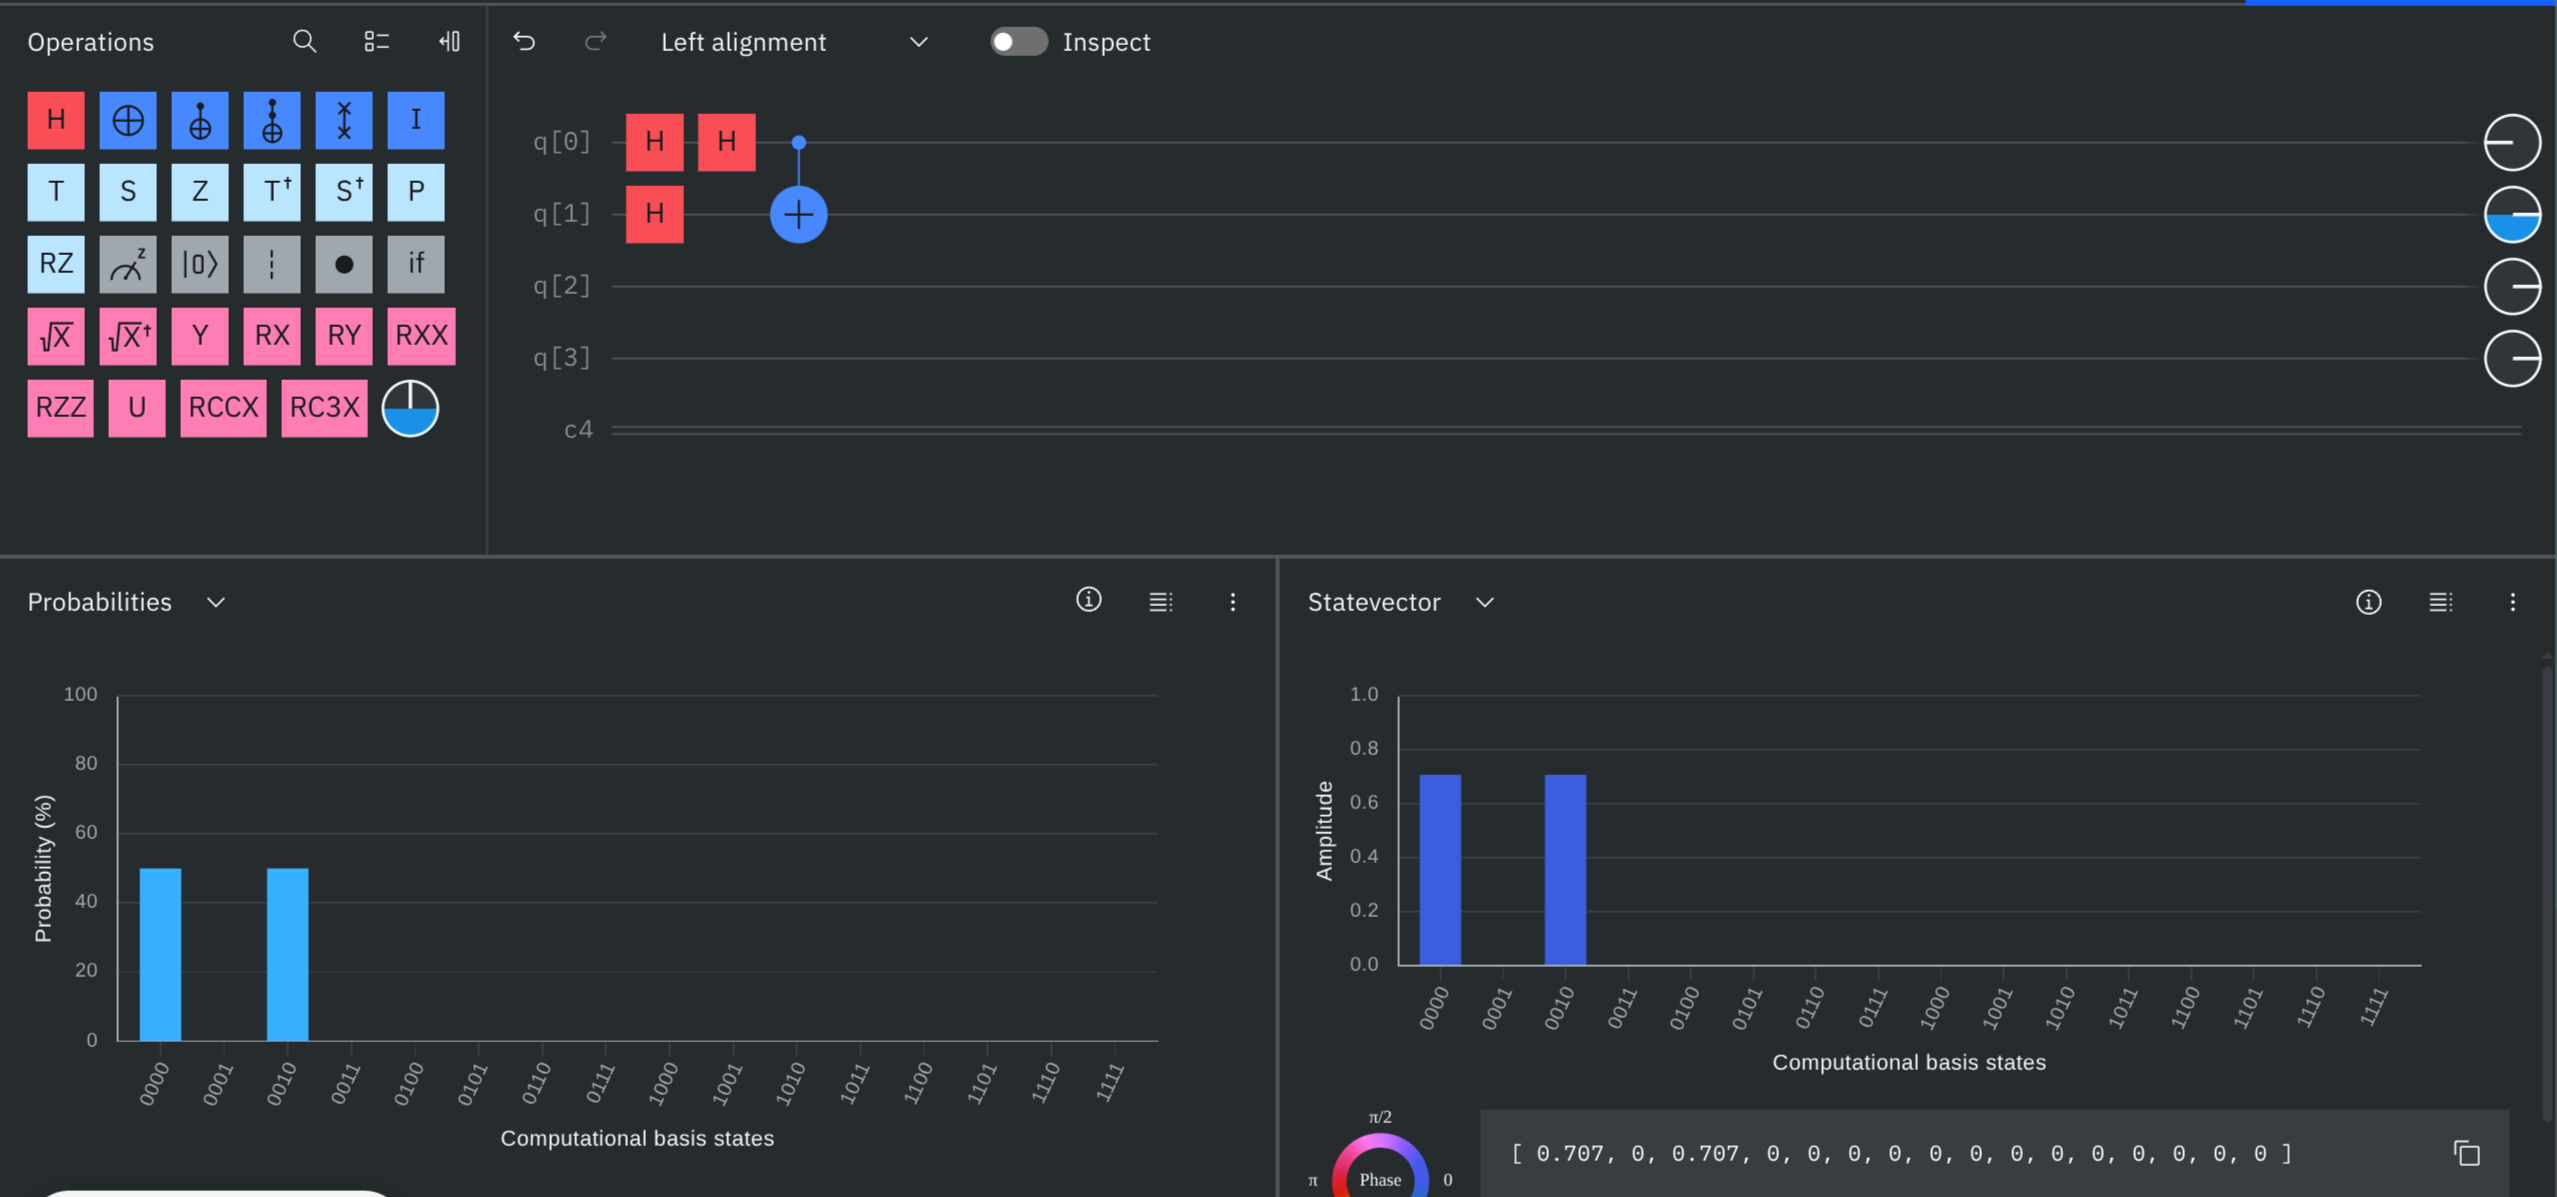
\includegraphics[width=\linewidth]{imgs/p3.png}

\end{document}
